%\documentclass[a4paper,11pt]{article}
\documentclass[a4paper,11pt]{scrartcl}

\usepackage[utf8]{inputenc}
\usepackage[italian]{babel}

\usepackage{graphicx} %for includng images
\graphicspath{{img/}}

\usepackage{siunitx} % package for deciBel and other units

\usepackage{amsmath} % package for ``cases'' and other matemagical stuff

\title{Appunti di compatibilità elettromagnetica}
\author{Daniele Olivieri}
\date{}

\pdfinfo{%
  /Title    ()
  /Author   ()
  /Creator  ()
  /Producer ()
  /Subject  ()
  /Keywords ()
}
\includeonly{lezione04_20_03}
\begin{document}
\maketitle

\section{Cenni sulla compatibilità elettromagnetica}
\paragraph{Definizione}
La compatibilità elettromagnetica è la scienza che studia la capacità di qualsiasi 
apparecchiatura di funzionare in modo soddisfacente in un ambiente soggetto a disturbi elettromagnetici
senza produrre disturbi intollerabili ad altri apparati.

Ad esempio quando si avvicina il cellulare alle casse dello stereo, si percepisce un ronzio nella cassa
dello stesso, questo fenomeno è dovuto al trasferimento di parte dell'energia emessa dal cellulare ai cavi 
dello stereo che lo convertono in disturbo sonoro.
Questo fenomeno non può e non deve avvenire nemmeno in situazioni critiche come una sala ospedaliera in cui il disturbo
emesso da un cellulare potrebbe alterare le misurazioni effettuate da un apparecchio come l'elettrocardiografo.
Il dispositivo elettromedicale deve essere reso immune dai disturbi. (Immagina un pacemaker!)

Si distingue la Compatibilità in senso attivo o passivo:
\begin{itemize}
 \item Attivo: l'oggetto non deve emettere disturbi di entità troppo elevata
 \item Passivo: l'oggetto deve essere in grado di resistere ai disturbi esterni, emessi da altri dispositivi
 senza alterare il proprio funzionamento
\end{itemize}

Altri dispositivi che devono sottoporsi alle analisi di Compatibilità sono i dispositivi comunque complessi
composti ad esempio da parti multiple, che possono essere commercializzate separatamente. In questo caso solo
le singole parti devono garantire un soddisfacimento dei vincoli dati dalla Compatibilità Elettromagnetica.

Si parla di Compatibilità \textbf{intra-sistema} se si analizza il problema all'interno del sistema con approccio
``microscopico'', la compatibilità \textbf{inter-sistema} analizza invece la compatibilità tra dispositivi differenti.
Esistono due grandi fenomeni: \textbf{emissione} e \textbf{immunità}, questi due fenomeni richiamano la compatibilità in senso attivo e passivo.
\medskip

I disturbi vengono poi caratterizzati in disturbi \textbf{radiati} in aria e disturbi \textbf{condotti} tramite
un canale vincolato, ad esempio un cavo di alimentazione.
Nessun disturbo si può caratterizzare mediante una singola tipologia, %rivedi qui
un disturbo radiato ad esempio può accoppiarsi con il cavo di alimentazione e diventare disturbo condotto.
Il cilindro di ferrite presente su un cavo VGA ad esempio attenua i disturbi che tendono a propagarsi lungo il cavo
incrementandone l'impedenza.
\newpage
Al di sotto dei 30 MHz si ritiene che il fenomeno sia di natura prevalentemente condotta,
al di sopra invece si ritiene il fenomeno di natura radiata. Ad esempio il ``\textbf{surge}'' nasce da un fulmine e si
propaga per via radiata, ma raggiunge i dispositivi mediante i loro cavi di alimentazione.

I problemi di compatibilità intra-sistema vengono gestiti durante la fase di progettazione del dispositivo
ad esempio mediante una corretta disposizione delle piste del circuito, attraverso una opportuna scelta dei 
componenti oppure mediante una schermatura interna, non disporrò mai un dispositivo molto suscettibile
in prossimità di un potenziale emettitore di disturbi sulla stessa scheda elettronica.

La compatibilità inter-sistema viene studiata mediante una caratterizzazione dell'ambiente elettromagnetico, 
mediante una classificazione delle sorgenti dei disturbi e delle vittime, attraverso la definizione dei livelli di massima
emissione e minima immunità, non riguarda soltanto l'oggetto ma anche la sua posizione nell'ambiente
elettromagnetico.
\medskip

L'\textbf{ambiente elettromagnetico} è l'insieme di tutti i fenomeni elettromagnetici osservabili in un
determinato luogo, sostanzialmente il \textbf{campo} elettromagnetico, le condizioni al contorno e le caratteristiche
del mezzo in cui i disturbi si propagano. Per modellare l'ambiente e ottenere un risultato valido
è necessaria una esatta conoscenza di tutti questi parametri, impresa per nulla semplice.

Anzichè calcolare la soluzione numericamente, si preferisce infatti misurare direttamente l'ambiente
elettromagnetico e le emissioni generate dall'oggetto. Anche quest'aspetto presenta dei problemi come
l'incertezza di misura e la discretizzazione del fenomeno, ovvero la scelta del numero di punti in cui effettuare
la misura.
Si può scegliere di eseguire entrambe le procedure, utilizzare un modello numerico approssimato per 
prevedere a grandi linee i risultati e approfondire con le misurazioni i punti più critici.

\paragraph{La perturbazione elettromagnetica}
È un fenomeno di origine elettromagnetico capace di alterare il funzionamento di un'apparecchiatura,
può essere costituito da:
\begin{itemize}
\item Rumore
\item Segnale non desiderato
\item Alterazione del mezzo
\end{itemize}


\section{Un pò di storia}
%\paragraph{}
A partire dal 1920 si diffondono i primi articoli riguardanti le interferenze radio, dando il via alla ricerca
sui problemi di compatibilità elettromagnetica.
Dieci anni dopo, con lo sviluppo delle industrie che utilizzavano energia elettrica si sono evidenziati i fenomeni
di disturbo e interferenza dovuti alle linee elettriche ferroviarie e all'utilizzo dei motori elettrici.
Durante la II Guerra Mondiale l'utilizzo di comunicazioni radio e sistemi radar fu cruciale per la riuscita
delle missioni, iniziò una vera e propria guerra tecnologica e ci si rese conto della necessità di regolamentare
le trasmissioni sulle varie frequenze.

Tra gli anni '50 e '70 si diffusero i transistor e l'elaborazione digitale dei dati, i circuiti divenivano
sempre più piccoli e commutavano a frequenze sempre più elevate. Questi segnali ad alte frequenze generavano numerosi
disturbi a banda larga in spazi molto ravvicinati fra i vari componenti.

\paragraph{Timeline essenziale} della compatibilità elettromagnetica:

\begin{itemize}
 \item \textbf{1923}: Primi rapporti tecnici sulle interferenze radio
 \item \textbf{1933}: Prime riunioni internazionali per la regolamentazione delle radio interferenze, IEC-UIR
 \item \textbf{1934}: Costituzione del CISPR, con prima riunione a Giugno
 \item \textbf{1979}: Documento da parte della FCC per la limitazione delle emissioni EM dei dispositivi digitali
\end{itemize}


In \textbf{Europa}: 
\begin{itemize}
 \item \textbf{1989}: Direttiva 89/336 in cui si obbligavano i produttori ad occuparsi della 
 Compatibilità Elettromagnetica, modificata da direttive successive nel 92, 93 ed entrò definitivamente in vigore
 nel Gennaio del 1996.
 \item \textbf{1996}: Recepimento in \textbf{Italia} con Decreto Legislativo n° 615.
 \item \textbf{1997-1998}: Pubblicazione delle \textit{guide di applicazione} UE e CEI per interpretare la Direttiva
 Europea.
 \item \textbf{CT 210}: Viene costituito il comitato tecnico 210 nel CENELEC e nel CEI riguardo la compatibilità
 elettromagnetica.
 \item \textbf{108/04/CE}: Direttiva a valle del progetto \textit{SLIM} al fine di semplificare la legislazione.
\end{itemize}

\paragraph{La direttiva Europea}
Documento mediante il quale l'Unione regola il commercio nel Mercato Interno, il produttore di un'apparecchiatura
deve fornire una \textit{``Dichiarazione di Conformità''} contenuta nel \textit{``Technical Construction
File''} che descriva il prodotto e ne illustri la conformità al fine di ottenere il marchio \textbf{CE}.

Nel \textit{1997} l'iniziativa nota come \textbf{SLIM} (Simplified Legislation for the Internal Market)
evidenziò la necessità di semplificare le normative mantenendo comunque un elevato livello di sicurezza.

Nel ``Nuovo Approccio'' la direttiva indica solo quali sono gli obiettivi da raggiungere ma non come farlo
per non limitare il progresso tecnologico. Le specifiche tecniche da rispettare vengono poi illustrate
nelle Norme Armonizzate, emanate da organizzazioni come il CENELEC, risulta in questo modo molto più semplice
aggiornare una Norma Armonizzata per modificare, ad esempio, i range di frequenza piuttosto che agire sull'intera 
Direttiva Europea, che richiederebbe un lavoro politico e burocratico molto più intenso.

\section{Gli apparati coinvolti}
L'articolo 2.1 della direttiva 108/04/CE distingue:
\begin{itemize}
 \item \textbf{Apparecchiatura}: Ogni apparecchio o impianto fisso
 \item \textbf{Apparecchio}: Dispositivo finito o combinazione di dispositivi finiti, commercializzati come unità 
 funzionali e destinati all'utente finale
 \item \textbf{Impianto fisso}: Combinazione particolare di apparecchi assemblati ed installati per essere
 utilizzati in un solo luogo
\end{itemize}

I dispositivi interessati coprono una grande varietà di settori, a partire dagli elettrodomestici agli apparecchi
per l'informazione, gli apparati per l'illuminazione, le macchine industriali fino alle apparecchiature 
elettromedicali.

La verifica della conformità \textbf{EMC} viene eseguita seguendo le Norme Armonizzate e il risultato delle prove viene
riportato nel \textit{Technical Construction File}, i prodotti che rispettano gli standard di prodotto, (o in assenza
di questi gli standard generici) vengono ritenuti conformi alla direttiva EMC e per questo viene prodotta la
dichiarazione di conformità e rilasciato il marchio CE.
Non è richiesta la marchiatura CE per le installazioni fisse dato che non devono essere commercializzate
tra i paesi membri ma devono solo garantire il corretto funzionamento nel punto in cui vengono installate.
La dichiarazione di conformità può prevedere una autocertificazione o l'intervento di un'autorità esterna per la
revisione della documentazione.

La differenza fra l'autocertificazione o l'intervento dell'autorità esterna è determinata dalla criticità del settore
in cui l'apparecchiatura deve funzionare (es. ambienti medicali, militari ecc...).

La verifica della conformità alla Direttiva EMC non solo consente il libero scambio di prodotti nel mercato europeo
ma permette comunque di realizzare un prodotto di livello superiore, con una maggiore robustezza ai disturbi e una
maggiore compatibilità anche in ambienti elettricamente ``affollati''.

\section{Gli organismi coinvolti}
Nel controllo del rispetto della Direttiva Europea sono coinvolti numerosi organismi e autorità:
Le \textbf{Autorità Competenti} sono enti riconosciuti dai singoli stati ai quali è stato affidato il compito
di vigilare sul mercato e controllare i prodotti che vi transitano, ad esempio le \underline{Camere di commercio}

Gli \textbf{Organismi Competenti} dimostrano di avere le competenze tecniche per verificare le caratteristiche di un 
apparato. Non eseguono le misurazioni sugli apparecchi ma sono in grado di analizzare e valutare
i risultati delle stesse.

Gli \textbf{Organismi Notificati} a cui è demandata, da parte delle Autorità Competenti, la verifica delle
caratteristiche di conformità alla direttiva EMC mediante le misure. Le certificazioni rilasciate dagli organismi
notificati sono già ritenute valide dalla Comunità Europea.

Un organismo competente o notificato deve avere disponibilità di attrezzatura specifica e personale specializzato,
non deve avere alcun conflitto di interessi con l'azienda che richiede la certificazione; deve essere sottoposto a 
verifica periodica. Le sue dichiarazioni hanno validità legale e deve essere assicurato sulla responsabilità civile
delle proprie dichiarazioni.

\begin{figure}[h]
 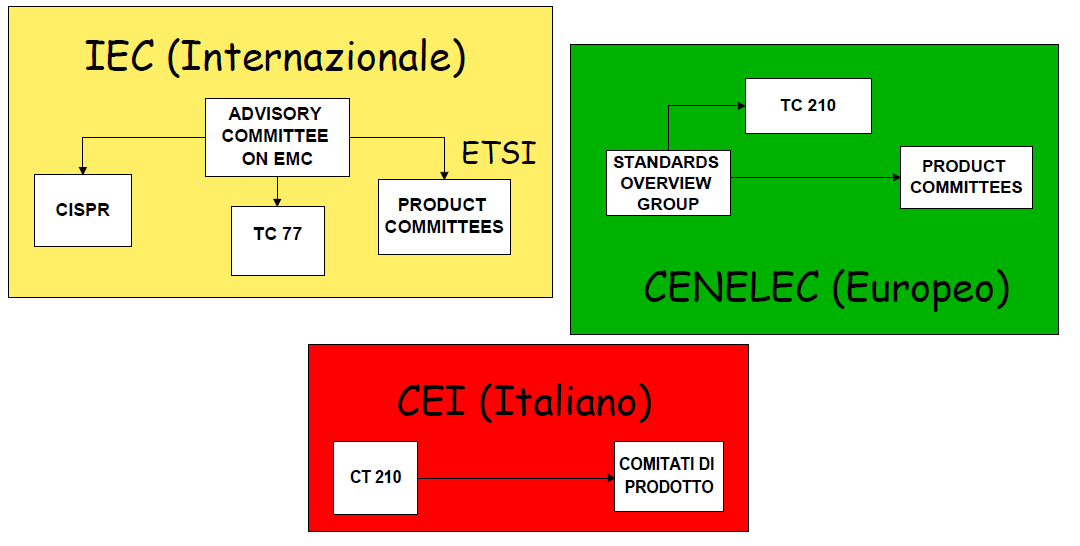
\includegraphics[width=0.7\linewidth]{enti.png}
 \centering
 \caption{Organismi di Normazione}
 \label{fig:enti}
\end{figure}

Tutti i paesi interessati partecipano all'IEC, le Norme attuate in Europa vengono invece rilasciate dal CENELEC mentre
il CEI in Italia collabora con i comitati di prodotto per redigere le norme.
L`IEC non è gerarchicamente superiore al CENELEC, nonostante sia un comitato internazionale non ha potere
sull'Europa, deve essere il CENELEC a recepire ed armonizzare una eventuale norma rilasciata dall'IEC.
L'Italia può avere una propria normazione tecnica ma se ci dovessero essere norme in contrasto con le normative 
Europee, queste dovranno essere aggiornate ed adeguate alla normazione più generale (europea). In teoria il singolo
Stato potrebbe avere normative più stringenti, ma queste potrebbero portare a ricorsi da parte dei produttori
che non potrebbero vendere i loro prodotti nei determinati stati membri, nonostante siano ``a norma''
secondo la Comunità Europea.

\paragraph{Il CISPR} È la commissione internazionale sui radiodisturbi, composta da vari sottocomitati: A,B,D,F,H,I.
%aggiungi elenco
\begin{itemize}
 \item \textbf{CISPR A}: Misure di interferenze radio e metodi statistici di misura.
 \item \textbf{CISPR B}: Interferenze dovute ad apparecchi industriali, scientifici, medicali, apparecchi ad alta tensione e
 apparecchi destinati alla mobilità elettrica.
 \item \textbf{CISPR D}: Disturbi dovuti a strumentazione elettrica/elettronica presente sui veicoli e tutti i dispositivi
 alimentati da motori a combustione interna.
 \item \textbf{CISPR F}: Interferenze dovute ad apparecchi domestici, attrezzi, illuminazione e apparecchi simili.
 \item \textbf{CISPR H}: Limiti per la protezione dei servizi radio.
 \item \textbf{CISPR I}: Compatibilità elettromagnetica per la protezione dei dispositivi IT, apparati e ricevitori 
 multimediali e simili.
\end{itemize}





\section{Enti normativi}
Il \textbf{CENELEC} è il comitato europeo di normazione elettrotecnica, in Italia invece l'ente normativo
è il \textbf{CEI}, Comitato Elettrotecnico Italiano che recepisce le normative europee e in genere le recepisce
traducendole senza apportare alcuna modifica, se il CEI ha invece già emanato una norma sull'argomento deve 
subito provvedere ad aggiornarla per renderla conforme con la normativa CENELEC, solitamente viene recepita
direttamente la norma CENELEC, ritirando quella italiana.

\textbf{Tipi di norme:}
\begin{itemize}
 \item \textbf{Base}: prettamente metodologica, descrizione della metodologia di prova, della strumentazione di misura
 con le sue caratteristiche, calibrazione dello stesso e ulteriori prescrizioni sui metodi di misura
 durante la validazione dell'elemento in prova. Non fissa alcun limite.
 \item \textbf{Generiche}: forniscono dei limiti e differenziano gli ambienti in cui i dispositivi vengono 
 utilizzati, ad esempio la suddivisione tra ambiente domestico, dove i dispositivi possono essere molto vicini
 tra loro, e l'ambiente industriale dove i dispositivi sono posti a distanze ragionevoli ed inoltre l'industria
 o l'azienda possiedono i fondi necessari alla ricerca di eventuali problemi di compatibilità.
 \item \textbf{Di prodotto}: fissano anch'esse dei limiti ma riguardano singoli prodotti o categorie di prodotti.
 Se per un prodotto non esiste una specifica norma, si applica la norma generica.
 \item \textbf{Armonizzate}: sono norme generiche o di prodotto, fatte proprie dall'unione europea e recepite,
 ``armonizzate'' dai vari stati includendole nel loro corpus normativo.
 \end{itemize}

Non sempre è necessario eseguire prove normate, ci si può affidare ad organismi terzi per verificare
il soddisfacimento dei requisiti. È possibile inoltre dimostrare la compatibilità elettromagnetica del proprio
prodotto utilizzando unicamente il progetto, se questo è in grado di dimostrare intrinsecamente il 
soddisfacimento dei requisiti imposti. È comunque preferito molto spesso l'approccio sperimentale per
la difficoltà molto spesso di avere un modello che copra tutti i range di frequenze.

Il CENELEC fu fondato nel '73 e composto dai comitati tecnici dei singoli paesi europei, inclusi affiliati
esterni che partecipano alle discussioni ma senza diritto di voto, è finalizzato all'armonizzazione: raccoglie 
ed elabora le norme emesse da altri enti (es. IEC) al fine di garantire uno standard richiesto dal mercato
europeo.

L'origine di una norma si riconosce mediante la sua sigla, ad esempio EN 50157-2-1.
\newpage
Le normative europee sono così numerate:
\begin{itemize}
 \item \textbf{40000/44999} derivano da una standardizzazione congiunta del CEN e del CENELEC riguardo
 il settore IT.
 \item \textbf{45000/49999} riguardano le attività congiunte CEN e CENELEC al di fuori del settore IT.
 \item \textbf{50000/59999} riguardano le attività esclusive del CENELEC.
 \item \textbf{60000/69999} l'implementazione da parte del CENELEC delle norme IEC.
\end{itemize}
Ad esempio la normativa europea EN 61000-4-3 deriva dalla IEC 1000-4-3 con le eventuali modifiche, la 
norma CISPR-16 è stata recepita in Europa con il numero EN 55016. 

\section{Approccio al problema}
Come ci si approccia al problema della compatibilità? Esiste l'approccio di \textbf{crisi}: si tenta di risolvere il
problema di compatibilità solo in fase di collaudo finale, senza tenere precedentemente in considerazione
eventuali problemi.
Questo approccio è molto rischioso dato che eventuali costi connessi alla soluzione saranno molto elevati
a causa della necessità di agire su un prodotto finito.

L'alternativa è l'approccio \textbf{sistematico}, ossia la considerazione dei problemi di compatibilità sin dalle fasi iniziali
della progettazione del prodotto, in questo modo è possibile risparmiare sui costi agendo in maniera tempestiva
su eventuali problemi e senza dover ritardare il rilascio del prodotto sul mercato.
Eventuali soluzioni potrebbero essere lo spostamento di una pista o l'allontanamento di due parti sensibili,
tutte queste procedure, in fase di progetto, sono economiche da applicare.
Questa tipologia di approccio prevede inoltre l'esecuzione di molteplici verifiche intermedie, a partire
da soluzioni simulate con un modello matematico fino a prove dirette sui prototipi iniziali.
\begin{figure}[h]
 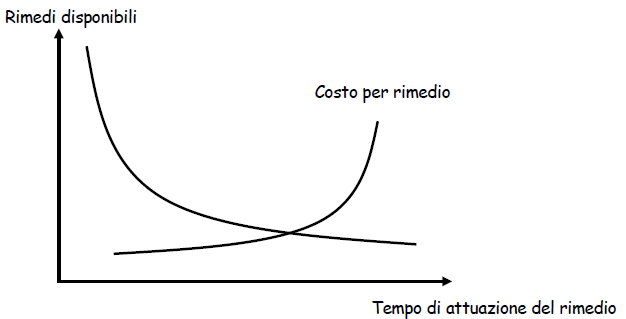
\includegraphics[width=0.7\linewidth]{costo_rimedio.png}
 \centering
 \caption{Rappresentazione del costo per rimedio in funzione del tempo di attuazione}
 \label{fig:costo_rimedio}
\end{figure}
%\newpage
Se il sistema è complesso si può dividere la scheda in più sezioni e analizzare le singole parti,
semplificando le analisi.

Gli ``attori'' che partecipano al fenomeno della compatibilità elettromagnetica sono sicuramente
almeno due: la \textbf{sorgente} e la \textbf{vittima}, tra i due è interposto il canale di accoppiamento.
Il disturbo può colpire la vittima mediante varie \textit{porte} come le porte di comunicazione,
di alimentazione o la porta ``involucro''.

I \textit{canali di accoppiamento} sono le vie utilizzate dai disturbi o dai segnali utili per propagarsi tra i 
dispositivi, il cavo di alimentazione può trasmettere disturbi al dispositivo provenienti dalla rete di alimentazione
ma può essere comunque protetto con un filtro, il discorso si complica per i canali di accoppiamento non previsti,
ovvero canali che non dovrebbero trasmettere alcuna informazione o energia utile per l'apparecchio.

\begin{figure}[h]
 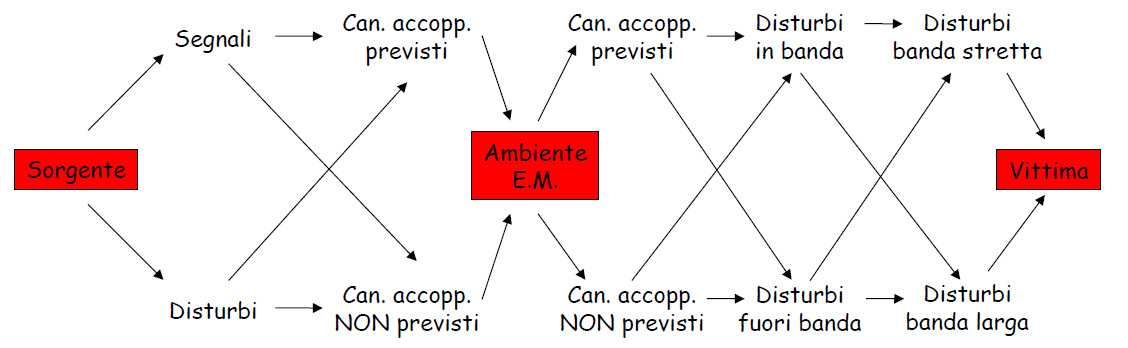
\includegraphics[width=0.7\linewidth]{catena_disturbi.png}
 \centering
 \caption{Rappresentazione della catena dei canali di accoppiamento dei disturbi}
 \label{fig:catena_disturbi}
\end{figure}

I disturbi che si propagano nella vittima possono rientrare o meno nella sua \textbf{banda} di funzionamento
ossia l'intervallo di frequenze alle quali è previsto il funzionamento del dispositivo, un disturbo si dice
a \textit{banda stretta} se rientra nella banda di funzionamento del dispositivo, si dice a \textit{banda larga}
se la sua ampiezza supera la banda di funzionamento del dispositivo.
Un disturbo a banda stretta (\textit{NarrowBand}) probabilmente potrà accoppiarsi con il dispositivo mediante
canali di accoppiamento previsti e risultare udibile per l'utente (ad esempio nel caso di un disturbo radiato che colpisce
un ricevitore FM).
Un disturbo a banda larga (\textit{BroadBand}) non rientra nelle caratteristiche di funzionamento del dispositivo
e potrà utilizzare con buona probabilità anche canali non previsti.
Un segnale composto da una singola componente in frequenza è un segnale a banda stretta per antonomasia.
\begin{figure}[h]
 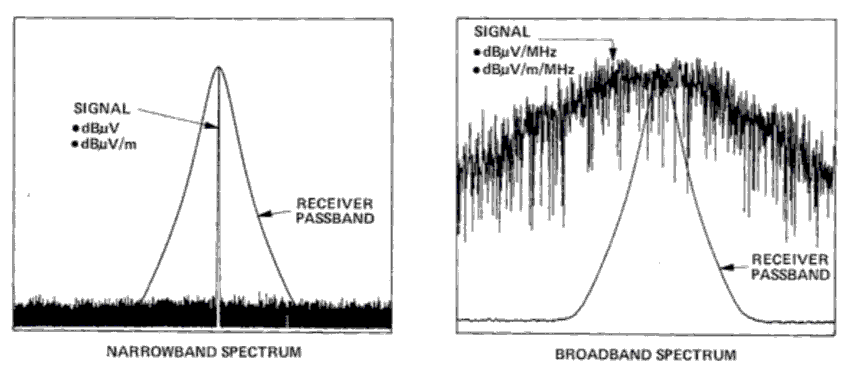
\includegraphics[width=0.7\linewidth]{narrow-broadband.png}
 \centering
 \caption{Confronto tra segnali a banda stretta e larga rispetto al filtro di un ricevitore}
 \label{fig:narrow-broadband}
\end{figure}








\section{Le unità di misura}
Le grandezze di interesse nel campo della Compatiiblità Elettromagnetica sono prevalentemente
campi elettrici [V/m] e magnetici [A/m], e tensioni [V] e correnti [I].
Queste grandezze variano con valori compresi tra $10^{-6}$ e $10^{2}$. C'è una dinamica di ben 8 ordini di grandezza.

Per gestire range così elevati, viene spesso utilizzata la rappresentazione su scale \textit{logaritmiche}.
Proprietà utili del logaritmo sono le seguenti:
\begin{itemize}
 \item [] Somma e differenza: $Y = aX/b \Rightarrow \log(Y) = \log(a) + \log(X) - \log(b) $
 \item [] Prodotto per uno scalare: $Y = 10^x \Rightarrow \log(Y) = x\log(10) $
\end{itemize}

È stato poi introdotto il ``decibel'' definito come:
$$\si{dB}(x) = 10\log_{10}x $$
Spesso si utilizza il deciBel per esprimere un guadagno o un'attenuazione di un amplificatore o un'antenna,
questa unità rappresenta quindi il rapporto tra due grandezze, in genere uscita e ingresso.
Se si indica un rapporto fra potenze continua a valere la precedente definizione ma per comodità
se la resistenza di ingresso dell'amplificatore e quella in uscita hanno lo stesso valore, si può ricavare
la seguente forma del deciBel più comoda e valida solo per le tensioni:

$$G_{P,\si{dB}} = 10\log_{10}\left(\frac{P_{out}}{P_{in}} \right) = 
10\log_{10}\left( \frac{V_{out}^2}{R_{out}}\frac{R_{in}}{V_{in}^2} \right) \stackrel{R_{in} = R_{out}}{=}
20\log_{10}\left(\frac{V_{out}}{V_{in}}\right) = G_{V,\si{dB}} $$

L'ampiezza della dinamica, utilizzando il deciBel diventa:
$$10^8 \Rightarrow 20\log_{10}10^8 = 160$$
in questo modo è molto più semplice rappresentare tali valori su una scala o un grafico.
Storicamente l'utilizzo del deciBel è nato dalla necessità dei costruttori di dispositivi audio di indicare
i livelli di volume sonoro e disturbo dato che anche l'orecchio umano percepisce i suoni con una funzione
logaritmica, tendendo ad attenuare i volumi elevati.

Altre forme del deciBel utilizzate sono quelle che fanno riferimento ad un valore fisso,
ad esempio il $\si{dB}\mu V = 20\log_{10}\frac{V}{1 \mu V}$ si indica quindi in deciBel, quanto la tensione
misurata è più grande (o più piccola) rispetto al \textit{microVolt}.

Per le potenze è spesso utile il $\si{dB}mW $ abbreviato $\si{dB}m = 10\log_{10}\frac{W}{1 mW}$.

\paragraph{Esempio potenza in antenna}
Potenza fornita ad un'antenna in funzione del campo elettrico emesso
$$P_T = G_T \frac{\lambda^2}{4\pi}\frac{E_T^2}{Z_0}$$
Supponiamo una variazione di $6 \si{dB}$ della potenza in antenna, a quanto corrisponde numericamente?
$$6\si{dB} = 10\log_{10}\left(\frac{P_2}{P_1} \right) = 10\log_{10}\left(\frac{E_2}{E_1}\right)^2 =
20\log_{10}\left(\frac{E_2}{E_1}\right) \Rightarrow$$

$$\Rightarrow
\begin{cases}
P_2 = 10^{\frac{6}{10}}\cdot P_1 \approx 4\cdot P_1 \\
E_2 = 10^{\frac{6}{20}}\cdot E_1 \approx 2\cdot E_1
\end{cases}
$$

Il guadagno è sempre adimensionale perchè esprime il rapporto tra grandezze identiche.

\paragraph{Propagazione in linea di trasmissione}





\end{document}
